% ============================================================
%  Internship Report — Unified Mentor Pvt. Ltd.
%  Rahul Vijay | Machine Learning Intern | 2025-2026
%  Compiled with: xelatex
% ============================================================
\documentclass[12pt, a4paper]{report}

% ── Core packages ────────────────────────────────────────────
\usepackage{fontspec}
\usepackage[top=1in, bottom=1in, left=1in, right=1in]{geometry}
\usepackage{graphicx}
\usepackage{xcolor}
\usepackage{setspace}
\usepackage{tabularx}
\usepackage{booktabs}
\usepackage{multirow}
\usepackage{array}
\usepackage{longtable}
\usepackage{titlesec}
\usepackage{fancyhdr}
\usepackage[hidelinks]{hyperref}
\usepackage{caption}
\usepackage{float}
\usepackage{tikz}
\usepackage{pgfplots}
\usepackage{parskip}
\usepackage{enumitem}
\usepackage{microtype}
\usepackage{indentfirst}
\usepackage{amsmath}
\usepackage{adjustbox}
\usepackage{tcolorbox}

\usetikzlibrary{shapes.geometric, arrows.meta, positioning, calc, backgrounds, fit}
\pgfplotsset{compat=1.18}
\tcbuselibrary{skins, breakable}

% ── Fonts ────────────────────────────────────────────────────
\setmainfont{Times New Roman}
\newfontfamily\headerfont{Times New Roman}[BoldFont={Times New Roman Bold}]

% ── Colours ──────────────────────────────────────────────────
\definecolor{dsublue}{HTML}{0070C0}
\definecolor{umblue}{HTML}{1E3A5F}
\definecolor{lightblue}{HTML}{EBF4FF}
\definecolor{tableheadblue}{HTML}{2E75B6}
\definecolor{lightgray}{HTML}{F5F5F5}
\definecolor{accentgray}{HTML}{CCCCCC}
\definecolor{darktext}{HTML}{2C2C2C}
\definecolor{greenbar}{HTML}{4CAF50}
\definecolor{yellowbar}{HTML}{FFC107}
\definecolor{redbar}{HTML}{F44336}

% ── Page style ───────────────────────────────────────────────
\pagestyle{fancy}
\fancyhf{}
\fancyhead[L]{\small\textit{Internship Report\,--\,Unified Mentor Pvt.\ Ltd.}}
\fancyhead[R]{\small\textit{Rahul Vijay}}
\fancyfoot[C]{\thepage}
\renewcommand{\headrulewidth}{0.4pt}
\renewcommand{\footrulewidth}{0pt}

\fancypagestyle{plain}{%
  \fancyhf{}%
  \fancyfoot[C]{\thepage}%
  \renewcommand{\headrulewidth}{0pt}%
}

% ── Chapter & section style ───────────────────────────────────
\titleformat{\chapter}[display]
  {\normalfont\Large\bfseries\centering}
  {\chaptertitlename\ \thechapter}{10pt}{\LARGE\bfseries}
\titlespacing*{\chapter}{0pt}{-10pt}{30pt}

\titleformat{\section}{\normalfont\large\bfseries}{\thesection}{1em}{}
\titlespacing*{\section}{0pt}{14pt}{6pt}

\titleformat{\subsection}{\normalfont\normalsize\bfseries}{\thesubsection}{1em}{}
\titlespacing*{\subsection}{0pt}{10pt}{4pt}

% ── Widow / orphan control ────────────────────────────────────
\widowpenalty=10000
\clubpenalty=10000

% ── Graphics path ─────────────────────────────────────────────
\graphicspath{{images/}}

% ── Table column types ────────────────────────────────────────
\newcolumntype{L}[1]{>{\raggedright\arraybackslash}p{#1}}
\newcolumntype{C}[1]{>{\centering\arraybackslash}p{#1}}
\newcolumntype{R}[1]{>{\raggedleft\arraybackslash}p{#1}}

\captionsetup{font=small, labelfont=bf, skip=8pt}

% ── Paragraph indent ─────────────────────────────────────────
\setlength{\parindent}{1.5em}

% ── TikZ styles ───────────────────────────────────────────────
\tikzset{
  layerbox/.style={rectangle, draw=umblue, fill=umblue!8,
    minimum width=13.5cm, minimum height=0.9cm, align=center, font=\small\bfseries},
  topbox/.style={layerbox, fill=umblue, text=white},
  confbox/.style={layerbox, fill=gray!15},
  procbox/.style={rectangle, rounded corners=4pt, draw=umblue, fill=umblue!10,
    text width=2.3cm, minimum height=1.2cm, align=center, font=\footnotesize},
  rawbox/.style={procbox, fill=gray!15, draw=gray},
  outbox/.style={procbox, fill=umblue!70, text=white, draw=umblue},
  myarrow/.style={-{Stealth[length=6pt]}, thick, color=umblue!70},
}

% ── Line spacing ─────────────────────────────────────────────
\setstretch{1.5}
\setlength{\headheight}{13.6pt}
\addtolength{\topmargin}{-1.6pt}
\tolerance=5000
\emergencystretch=3em

% =============================================================
\begin{document}

% =============================================================
%  COVER PAGE
% =============================================================
\newgeometry{top=0.9in, bottom=0.9in, left=0.9in, right=0.9in}
\thispagestyle{empty}
\begin{center}

  % ── Top logos ──────────────────────────────────────────────
  \begin{minipage}[c]{0.63\textwidth}
    \centering
    
\includegraphics[width=\textwidth]{cover_image3.png}
  \end{minipage}%
  \hfill%
  \begin{minipage}[c]{0.25\textwidth}
    \centering
    
\includegraphics[width=\textwidth]{cover_image1.jpeg}
  \end{minipage}

  \vspace{0.2cm}
  
\includegraphics[width=0.48\textwidth]{cover_image2.png}

  \vspace{0.15cm}
  {\rule{\textwidth}{1.5pt}}

  \vspace{0.2cm}
  {\normalsize Devarakaggalahalli, Harohalli, Kanakapura Road,
  South Bengaluru Dt., Karnataka\,--\,562112, India}

  \vspace{0.35cm}
  {\large An Internship Report on}

  \vspace{0.2cm}
  {\LARGE\bfseries\color{dsublue}
    Shipping Route Efficiency Analysis\\[4pt]
    for the Logistics Sector}

  \vspace{0.25cm}
  {\rule{\textwidth}{0.6pt}}

  \vspace{0.25cm}
  {\normalsize Submitted in Partial Fulfillment for the Award of Degree in}\\[6pt]
  {\large\bfseries Bachelor of Technology}\\[4pt]
  {\normalsize in}\\[4pt]
  {\large\bfseries COMPUTER SCIENCE AND ENGINEERING\\[2pt]
  (ARTIFICIAL INTELLIGENCE \& MACHINE LEARNING)}

  \vspace{0.45cm}
  {\normalsize\bfseries Submitted by}\\[6pt]
  {\large\textit{$\langle$STUDENT NAME$\rangle$}}\\[4pt]
  {\large\textit{$\langle$USN$\rangle$}}

  \vspace{0.35cm}
  {\normalsize\bfseries Internship carried out at}\\[4pt]
  {\large\bfseries\color{dsublue} Unified Mentor Pvt.\ Ltd.}\\[2pt]
  {\normalsize DLF Forum, Cybercity, Phase III, Gurugram, Haryana\,--\,122002}

  \vspace{0.4cm}
  \begin{tabular}{C{0.45\textwidth}C{0.45\textwidth}}
    \textbf{INTERNAL GUIDE} & \textbf{EXTERNAL GUIDE} \\[6pt]
    $\langle$\textit{Name}$\rangle$ & $\langle$\textit{Name}$\rangle$ \\[4pt]
    Assistant/Associate/Professor & $\langle$\textit{Designation}$\rangle$ \\[4pt]
    Dept.\ of CSE(AI\,\&\,ML), SoE, DSU &
      $\langle$\textit{Company Name, Location}$\rangle$ \\
  \end{tabular}

  \vfill

  {\rule{\textwidth}{1.5pt}}\\[6pt]
  {\normalsize\bfseries DEPARTMENT OF COMPUTER SCIENCE \& ENGINEERING (AI\,\&\,ML)}\\[2pt]
  {\normalsize\bfseries SCHOOL OF ENGINEERING}\\[2pt]
  {\large\bfseries DAYANANDA SAGAR UNIVERSITY}\\[2pt]
  {\normalsize BENGALURU, KARNATAKA \quad (2025\,--\,2026)}

\end{center}
\restoregeometry
\clearpage

% =============================================================
%  UNIVERSITY CERTIFICATE
% =============================================================
\newgeometry{top=0.4in, bottom=0.7in, left=0.89in, right=0.63in}
\thispagestyle{empty}
\begin{center}

  \begin{minipage}[c]{0.52\textwidth}
    \centering
    
\includegraphics[width=\textwidth]{cert_image1.png}
  \end{minipage}%
  \hfill%
  \begin{minipage}[c]{0.22\textwidth}
    \centering
    
\includegraphics[width=\textwidth]{cert_image2.jpeg}
  \end{minipage}

  \vspace{0.15cm}
  {\color{dsublue}\large\bfseries DAYANANDA SAGAR UNIVERSITY}\\[2pt]
  {\color{dsublue}\normalsize Department of Computer Science \& Engineering}\\[-2pt]
  {\color{dsublue}\normalsize (Artificial Intelligence \& Machine Learning)}\\[2pt]
  {\color{dsublue}\small
    Devarakaggalahalli, Harohalli, Kanakapura Road,
    South Bengaluru Dt., Karnataka\,--\,562112, India}

  \vspace{0.25cm}
  {\rule{\textwidth}{0.8pt}}

  \vspace{0.3cm}
  {\Huge\bfseries CERTIFICATE}
  \vspace{0.3cm}

\end{center}

{\setstretch{1.6}
This is to certify that the Internship report, entitled
\textbf{``\textit{$\langle$Title$\rangle$}''}, a bonafide student of
Bachelor of Technology in Department of Computer Science and Engineering
(Artificial Intelligence \& Machine Learning) at the School of Engineering,
Dayananda Sagar University, Bengaluru in partial fulfillment of the requirement
for the VIII Semester during the academic year 2025\,--\,2026.

It is certified that all the corrections/suggestions indicated for Internal
Assessment have been incorporated in the report. The Internship report has
been approved as it satisfies the academic requirements in respect of
Internship prescribed for the VIII Semester.
}

\vspace{0.6cm}

\noindent
\begin{tabular}{|C{0.31\textwidth}|C{0.31\textwidth}|C{0.31\textwidth}|}
\hline
\rule{0pt}{12pt}\textbf{External Guide} &
  \textbf{Internal Guide} &
  \textbf{Chairperson} \\[2pt]
\hline
\rule{0pt}{10pt}\textbf{Name} & \textbf{Name} & \textbf{Name} \\[2pt]
$\langle$\textit{Name}$\rangle$ &
  $\langle$\textit{Name}$\rangle$ &
  Dr.\ Jayavrinda Vrindavanam \\[4pt]
\hline
\rule{0pt}{10pt}\textbf{Designation} & \textbf{Designation} & \textbf{Designation} \\[2pt]
$\langle$\textit{Designation}$\rangle$ &
  Assistant/Associate/Professor &
  Professor \& Chairperson \\[4pt]
\hline
\rule{0pt}{10pt}\textbf{Company/Organization} &
  \textbf{Department} &
  \textbf{Department} \\[2pt]
$\langle$\textit{Company/Organization}$\rangle$ &
  Dept.\ of CSE(AI\,\&\,ML) &
  Dept.\ of CSE(AI\,\&\,ML) \\[4pt]
\hline
\rule{0pt}{10pt}\textbf{Location} & \textbf{School} & \textbf{School} \\[2pt]
$\langle$\textit{Location}$\rangle$ &
  School of Engineering, DSU &
  School of Engineering, DSU \\[4pt]
\hline
\rule{0pt}{10pt}\textbf{Date:} & \textbf{Date:} & \textbf{Date:} \\[22pt]
\hline
\end{tabular}

\restoregeometry
\clearpage

% =============================================================
%  DECLARATION
% =============================================================
\newgeometry{top=0.2in, bottom=1in, left=1.2in, right=1in}
\thispagestyle{empty}
\begin{center}

  \begin{minipage}[c]{0.52\textwidth}
    \centering
    
\includegraphics[width=\textwidth]{decl_image1.png}
  \end{minipage}%
  \hfill%
  \begin{minipage}[c]{0.22\textwidth}
    \centering
    
\includegraphics[width=\textwidth]{decl_image2.jpeg}
  \end{minipage}

  \vspace{0.2cm}
  {\color{dsublue}\large\bfseries DAYANANDA SAGAR UNIVERSITY}\\[2pt]
  {\color{dsublue}\normalsize Department of Computer Science \& Engineering}\\[-2pt]
  {\color{dsublue}\normalsize (Artificial Intelligence \& Machine Learning)}\\[2pt]
  {\color{dsublue}\small
    Devarakaggalahalli, Harohalli, Kanakapura Road,
    South Bengaluru Dt., Karnataka\,--\,562112, India}

  \vspace{0.3cm}
  {\rule{\textwidth}{0.8pt}}

  \vspace{0.4cm}
  {\Huge\bfseries DECLARATION}
  \vspace{0.4cm}

\end{center}

{\setstretch{1.6}
I, $\langle$\textit{NAME}$\rangle$, hereby declare that the Internship titled
\textbf{``$\langle$\textit{Title}$\rangle$''} embodied in this report has been
carried out by me during VIII Semester B.Tech in Computer Science and Engineering
(Artificial Intelligence \& Machine Learning), at School of Engineering,
Dayananda Sagar University, submitted in partial fulfillment for the award of
degree in Bachelor of Technology in Computer Science and Engineering (Artificial
Intelligence \& Machine Learning) during the academic year 2025\,--\,2026.

The work embodied in this report is original and it has not been submitted in
part or full for any other degree in any University.
}

\vspace{1.5cm}

\noindent
\rule{6cm}{0.4pt}\\[4pt]
$\langle$\textit{Name}$\rangle$\\
$\langle$\textit{USN}$\rangle$

\vspace{0.8cm}
\noindent Place\,:\enspace Bengaluru\\[4pt]
Date\,:\enspace\rule{3cm}{0.4pt}

\restoregeometry
\clearpage

% =============================================================
%  ACKNOWLEDGEMENT
% =============================================================
\thispagestyle{empty}
\begin{center}
  {\LARGE\bfseries ACKNOWLEDGEMENT}
\end{center}
\vspace{0.4cm}

\noindent\textit{It is a great pleasure for us to acknowledge the assistance and
support of many individuals who have been responsible for the successful
completion of this project work. First, I take this opportunity to express our
sincere gratitude to School of Engineering, Dayananda Sagar University,
Bengaluru, Karnataka, India for providing us with a great opportunity to pursue
our Bachelor's degree in this institution.}

\vspace{0.4cm}

\noindent\textit{I am highly elated in expressing my sincere and abundant respect
to \textbf{Dr.\ D.\ Hemachandra Sagar}, Chancellor, \textbf{Dr.\ D.\ Premachandra
Sagar}, Pro Chancellor, \textbf{Dr.\ B.\ S.\ Satyanarayana}, Vice Chancellor,
\textbf{Dr.\ C.\ Puttamadappa}, Registrar, \textbf{Dr.\ K.\ R.\ Udaya Kumar Reddy},
Dean, School of Engineering (SoE), Dayananda Sagar University, Bengaluru,
Karnataka, India for their constant encouragement and expert advice.}

\vspace{0.4cm}

\noindent\textit{It is a matter of immense pleasure to express my sincere thanks
to \textbf{Dr.\ Jayavrinda Vrindavanam}, Professor \& Department Chairperson,
Computer Science and Engineering (Artificial Intelligence \& Machine Learning),
Dayananda Sagar University, Bengaluru, Karnataka, India for providing right
academic guidance that made our task possible.}

\vspace{0.4cm}

\noindent\textit{I would like to thank our External guide
\rule{4cm}{0.4pt}, $\langle$\textit{Designation}$\rangle$,
$\langle$\textit{Company Address and Details}$\rangle$, for sparing his/her
valuable time to extend help in every step of our Internship work, which paved
the way for smooth progress and fruitful culmination of Internship.}

\vspace{0.4cm}

\noindent\textit{I would like to thank our Internal guide \rule{4cm}{0.4pt},
Associate/Assistant/Professor, Department of Computer Science and Engineering
(AI\,\&\,ML), Dayananda Sagar University, Bengaluru, Karnataka, India for
sparing his/her valuable time to extend help in every step of our Internship
work, which paved the way for smooth progress and fruitful culmination of
the Internship.}

\vspace{0.4cm}

\noindent\textit{I would like to thank our Internship Coordinator
\textbf{Dr.\ Joshuva Arockia Dhanraj}, Professor, Department of Computer
Science and Engineering (AI\,\&\,ML) as well as all the staff members of
Computer Science and Engineering (AI\,\&\,ML) for their support.}

\vspace{0.4cm}

\noindent\textit{I am also grateful to our family and friends who provided us
with every requirement throughout the course. I would like to thank one and
all who directly or indirectly helped us in the Internship Project work.}

\vspace{1.2cm}

\begin{flushright}
  \textit{\textbf{$\langle$Name$\rangle$}}\\[4pt]
  \textit{\textbf{$\langle$USN$\rangle$}}
\end{flushright}

\clearpage

% =============================================================
%  TABLE OF CONTENTS
% =============================================================
\thispagestyle{plain}
\begin{center}
  {\LARGE\bfseries CONTENTS}
\end{center}
\vspace{0.3cm}
\tableofcontents
\clearpage

% =============================================================
%  LIST OF FIGURES
% =============================================================
\listoffigures
\clearpage

% =============================================================
%  LIST OF TABLES
% =============================================================
\listoftables
\clearpage

% =============================================================
%  ABSTRACT  (roman page i)
% =============================================================
\pagenumbering{roman}
\setcounter{page}{1}
\chapter*{Abstract}
\addcontentsline{toc}{chapter}{Abstract}

This report documents the Machine Learning internship undertaken at
\textbf{Unified Mentor Pvt.\ Ltd.}, Gurugram, Haryana, from
25\textsuperscript{th} March 2026 to 25\textsuperscript{th} June 2026.
The internship was carried out in the Machine Learning and Data Analytics
domain, with the primary objective of developing an interactive, data-driven
analytics platform for a distribution sector client of the company.

The client required a system that could provide operational visibility into
the performance of a multi-factory, multi-region shipping network. The project
involved designing and implementing a complete data pipeline — from raw
transactional data ingestion and schema validation, through feature
engineering and analytics computation, to an interactive web dashboard
with ten embedded visualizations spanning four analytical perspectives.

The key technical contributions include: a cohort-based lead time normalization
algorithm that isolates a genuine 0--11 day efficiency signal from an otherwise
noisy 900--1{,}640 day lead time baseline; a min-max normalized route
efficiency scoring system; and a fully modular, production-ready Python
application architecture built on Streamlit, Pandas, Plotly, and pandera.
The application is supported by a suite of 28 automated unit tests.

The internship provided substantial professional development across both
technical (Python data stack, software architecture, testing, visualization)
and professional (client-focused problem solving, code quality, documentation)
dimensions. The resulting system was validated against the client's sample
dataset and is ready for deployment on actual operational data.

\clearpage

% =============================================================
%  COMPANY CERTIFICATE OF INTERNSHIP  (page 1, arabic)
% =============================================================
\pagenumbering{arabic}
\setcounter{page}{1}
\chapter*{Certificate of Internship}
\addcontentsline{toc}{chapter}{Certificate of Internship}
\thispagestyle{plain}

\vspace{0.5cm}

\begin{tcolorbox}[
  colback=lightblue,
  colframe=umblue,
  boxrule=1.5pt,
  arc=4pt,
  left=14pt, right=14pt, top=14pt, bottom=14pt
]
  \begin{center}
    {\Large\bfseries\color{umblue} UNIFIED MENTOR PVT.\ LTD.}\\[6pt]
    {\normalsize\color{umblue}
      DLF Forum, Cybercity, Phase III, Gurugram, Haryana\,--\,122002}\\[2pt]
    {\normalsize\color{umblue}
      Tel: +91 6283 800330 \quad|\quad www.unifiedmentor.com}
  \end{center}

  \vspace{0.5cm}

  {\setstretch{1.6}
  \noindent\textbf{Date:} 25/03/2026 \hfill
  \textbf{UNID:} UMID22303268609

  \vspace{0.4cm}
  \noindent\textbf{To Whom It May Concern,}

  \vspace{0.3cm}
  This is to certify that \textbf{Rahul Vijay} has successfully undertaken a
  Machine Learning Internship at Unified Mentor Pvt.\ Ltd.\ for a period of
  \textbf{3 months}, from \textbf{25\textsuperscript{th} March 2026} to
  \textbf{25\textsuperscript{th} June 2026}.

  During this period, the intern was engaged in the Machine Learning and Data
  Analytics domain and worked on a live project involving the design and
  development of a shipping route efficiency analytics platform for one of
  our distribution sector clients. The intern demonstrated strong initiative,
  technical aptitude, and professional conduct throughout the engagement.

  We wish Rahul Vijay the very best in all future endeavours.
  }

  \vspace{0.8cm}

  \noindent\rule{5cm}{0.4pt}\\[4pt]
  \textbf{Drishti Madaan}\\
  HR Manager, Unified Mentor Pvt.\ Ltd.\\
  Tel: +91 6283 800330 \quad|\quad info@unifiedmentor.com
\end{tcolorbox}

\clearpage

% =============================================================
%  CHAPTER 1 — ABOUT THE ORGANIZATION
% =============================================================
\chapter{About the Organization}

\section{Introduction}

Unified Mentor Pvt.\ Ltd.\ is an emerging Education Technology (EdTech) company
headquartered at DLF Forum, Cybercity, Phase III, Gurugram, Haryana\,--\,122002,
India. The company was established with a singular focus: to bridge the persistent
gap between what academic programmes teach and what industry actually expects from
fresh talent.

Unified Mentor operates through a \emph{project-driven internship model} where
students and early-career professionals are assigned live industry projects under
the guidance of experienced technical mentors. This approach departs from
conventional classroom-based learning and places the intern directly in the
role of a junior professional working on real-world deliverables with genuine
business impact.

The company's internship programme spans multiple technology domains, including
Machine Learning, Data Science, Full-Stack Web Development, Data Engineering, and
Business Analytics. Each project is sourced from an actual client requirement,
meaning that the intern's output contributes to a tangible product or service
rather than being a simulated exercise.

As of 2026, Unified Mentor has built a growing portfolio of client projects and
a network of mentors drawn from industry practitioners across India's major
technology hubs. The organisation maintains a lean, agile structure designed to
maximise the quality of mentorship and the depth of project engagement for every
intern.

\section{Vision}

The vision of Unified Mentor is to become a leading platform for practical,
industry-aligned technical education in India — one where the journey from
student to employable professional is direct, structured, and measurably
effective. The company aspires to be the preferred partner both for students
seeking meaningful internship experiences and for organisations seeking
well-prepared entry-level talent.

At its core, this vision rests on the belief that \emph{real learning happens
through real work}. By pairing motivated students with genuine client projects
and experienced mentors, Unified Mentor aims to compress the transition time
between graduation and productive employment.

\section{Mission}

The mission of Unified Mentor is to empower students and early-career
professionals through:

\begin{itemize}[leftmargin=1.5em, itemsep=4pt]
  \item \textbf{Live project engagement:} Every intern works on a real client
    project with defined deliverables, deadlines, and review cycles.
  \item \textbf{Expert mentorship:} Projects are supervised by industry
    professionals who provide technical guidance, code reviews, and
    career advice throughout the engagement.
  \item \textbf{Skill-based certification:} Interns who successfully complete
    their projects receive industry-recognised certificates that validate
    practical, demonstrable skills.
  \item \textbf{Affordable access:} The programme is structured to be
    accessible to students across diverse economic backgrounds.
  \item \textbf{Talent pipeline development:} By training a pipeline of
    project-ready professionals, the company supports the hiring goals of
    its client organisations.
\end{itemize}

\section{Team}

Unified Mentor operates with a structured team that balances programme
management, technical mentorship, and client relationship functions.
Figure~\ref{fig:orgchart} illustrates the organisational structure as
experienced during the internship.

\begin{figure}[H]
  \centering
  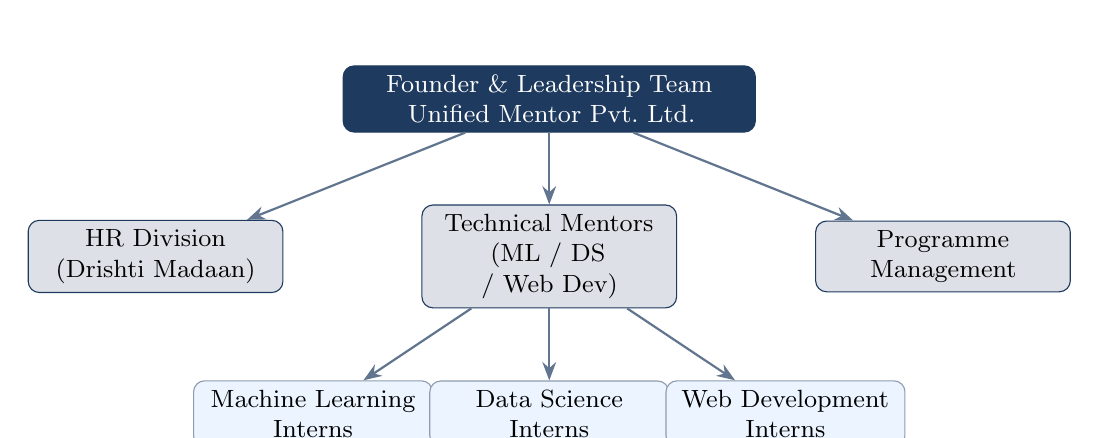
\begin{tikzpicture}[font=\small, >=Stealth,
    mgr/.style={rectangle, rounded corners=4pt, draw=umblue, fill=umblue,
      text=white, text width=3.6cm, minimum height=0.8cm, align=center},
    dept/.style={rectangle, rounded corners=4pt, draw=umblue, fill=umblue!15,
      text width=3.0cm, minimum height=0.8cm, align=center},
    intern/.style={rectangle, rounded corners=4pt, draw=umblue!50,
      fill=lightblue, text width=2.8cm, minimum height=0.8cm, align=center},
  ]
    \node[mgr, text width=5cm] (top) at (0,0) {Founder \& Leadership Team\\Unified Mentor Pvt.\ Ltd.};

    \node[dept] (hr)   at (-5,-2) {HR Division\\(Drishti Madaan)};
    \node[dept] (tech) at (0,-2)  {Technical Mentors\\(ML / DS / Web Dev)};
    \node[dept] (pm)   at (5,-2)  {Programme\\Management};

    \node[intern] (ml)  at (-3,-4) {Machine Learning\\Interns};
    \node[intern] (ds)  at (0,-4)  {Data Science\\Interns};
    \node[intern] (wd)  at (3,-4)  {Web Development\\Interns};

    \draw[->, thick, umblue!70] (top) -- (hr);
    \draw[->, thick, umblue!70] (top) -- (tech);
    \draw[->, thick, umblue!70] (top) -- (pm);
    \draw[->, thick, umblue!70] (tech) -- (ml);
    \draw[->, thick, umblue!70] (tech) -- (ds);
    \draw[->, thick, umblue!70] (tech) -- (wd);
  \end{tikzpicture}
  \caption{Organisational structure of Unified Mentor Pvt.\ Ltd.}
  \label{fig:orgchart}
\end{figure}

The HR division, headed by Drishti Madaan, manages intern onboarding, offer
letters, programme scheduling, and compliance. The technical mentors are domain
specialists who review project outputs and provide week-to-week guidance. The
programme management function coordinates client relationships, project scoping,
and delivery timelines.

\section{Services}

Unified Mentor's core service portfolio is summarised in Table~\ref{tab:services}.

\begin{table}[H]
  \centering
  \caption{Core services offered by Unified Mentor Pvt.\ Ltd.}
  \label{tab:services}
  \begin{tabularx}{\textwidth}{@{} L{0.25\textwidth} X @{}}
    \toprule
    \textbf{Service} & \textbf{Description} \\
    \midrule
    Live Internships &
      Structured 1--6 month engagements on real client projects; domains
      include ML, Data Science, Full-Stack Development, Data Engineering,
      and Business Analytics. \\[4pt]
    Certification Programmes &
      Skill-specific certification courses combining self-paced content
      with mentored project work; certificates are issued on successful
      completion. \\[4pt]
    Technical Mentorship &
      One-on-one and small-group sessions with industry practitioners
      covering project design, code review, and career strategy. \\[4pt]
    Skill Assessments &
      Domain-specific assessments used to match candidates to appropriate
      project tracks and to benchmark learning progress. \\[4pt]
    Placement Support &
      Resume building, mock interviews, and referral support for interns
      completing the programme. \\
    \bottomrule
  \end{tabularx}
\end{table}

% =============================================================
%  CHAPTER 2 — ABOUT THE DEPARTMENT
% =============================================================
\chapter{About the Department}

\section{Introduction}

Within Unified Mentor, the \textbf{Machine Learning and Data Analytics
Division} is responsible for client engagements that require data-driven
intelligence solutions. This division works across a spectrum of project
types — from exploratory data analysis and business intelligence dashboarding,
to predictive modelling, anomaly detection, and natural language processing
applications.

Interns assigned to this division are placed within project teams under the
direct supervision of a technical mentor who has industry experience in the
relevant domain. The division follows an agile, sprint-based delivery model,
with weekly mentor check-ins, fortnightly deliverable reviews, and a final
project demonstration at the end of the internship period.

The ML and Analytics division currently handles projects across industries
including retail, logistics, healthcare, finance, and e-commerce, providing
clients with purpose-built data products that convert raw operational data
into actionable intelligence.

\section{Employee Experience Department}

The employee (intern) experience function at Unified Mentor is designed to
ensure that every participant receives a structured, supportive, and
educationally rich engagement from day one. The typical onboarding and
project lifecycle is as follows:

\begin{enumerate}[leftmargin=1.5em, itemsep=6pt]
  \item \textbf{Onboarding (Week 1):}
    The intern receives their offer letter, UNID, and project brief from
    the HR division. An introductory session with the technical mentor
    covers project scope, deliverables, tool access, and development
    environment setup.

  \item \textbf{Exploration \& Planning (Weeks 2--3):}
    The intern explores the provided dataset or problem context, conducts
    background research, and submits an initial project plan. The mentor
    reviews the plan and provides feedback.

  \item \textbf{Development (Weeks 4--10):}
    The core development phase, structured in two-week sprints. Each
    sprint has defined deliverables. The mentor provides code review
    feedback via comments and synchronous sessions. The intern is
    expected to maintain clean, well-documented, testable code.

  \item \textbf{Review \& Refinement (Weeks 11--12):}
    The intern incorporates mentor feedback, prepares the final report,
    and conducts a project demonstration. The mentor verifies that all
    agreed deliverables have been met.

  \item \textbf{Certification \& Closure:}
    On successful completion, the intern receives their certificate and
    a letter of recommendation from the HR division.
\end{enumerate}

Communication throughout the internship is conducted via email and virtual
meeting platforms. The intern is expected to use version control (Git) for
all code submissions and to maintain a project log documenting weekly
progress.

\section{Analytics Project Development Process}

The ML and Data Analytics division at Unified Mentor follows a structured
project development methodology that mirrors the standards observed in
professional data engineering and data science teams. Figure~\ref{fig:devprocess}
illustrates this process.

\begin{figure}[H]
  \centering
  
\begin{tikzpicture}[font=\small, >=Stealth,
    pstep/.style={rectangle, rounded corners=5pt, draw=umblue, fill=umblue!12,
      text width=2.4cm, minimum height=1.4cm, align=center},
  ]
    \node[pstep] (n0) at (0,   0) {Client\\Brief \&\\Scoping};
    \node[pstep] (n1) at (2.6, 0) {Data\\Exploration\\(EDA)};
    \node[pstep] (n2) at (5.2, 0) {Architecture\\Design};
    \node[pstep] (n3) at (7.8, 0) {Development\\(Sprints)};
    \node[pstep] (n4) at (10.4,0) {Testing \&\\Validation};
    \node[pstep] (n5) at (13.0,0) {Delivery \&\\Handover};
    \draw[->, thick, umblue!70] (n0.east) -- (n1.west);
    \draw[->, thick, umblue!70] (n1.east) -- (n2.west);
    \draw[->, thick, umblue!70] (n2.east) -- (n3.west);
    \draw[->, thick, umblue!70] (n3.east) -- (n4.west);
    \draw[->, thick, umblue!70] (n4.east) -- (n5.west);
  \end{tikzpicture}
  \caption{Analytics project development process at Unified Mentor.}
  \label{fig:devprocess}
\end{figure}

Each stage is briefly described below:

\begin{description}[leftmargin=0pt, itemsep=6pt]
  \item[\textbf{Client Brief \& Scoping:}]
    The client's business problem is documented, key questions are identified,
    and data availability is assessed. Deliverables and timelines are agreed.

  \item[\textbf{Data Exploration (EDA):}]
    The provided dataset is examined for structure, quality, distributions,
    and anomalies. Findings inform the feature engineering strategy.

  \item[\textbf{Architecture Design:}]
    The technical architecture is designed before any code is written.
    Module boundaries, data flows, configuration strategy, and testing
    approach are all specified in advance.

  \item[\textbf{Development (Sprints):}]
    Code is written module-by-module, following the agreed architecture.
    Each module is unit-tested. The mentor reviews code at the end of
    each sprint.

  \item[\textbf{Testing \& Validation:}]
    The complete system is validated against the client's data. All unit
    tests are run. Performance, correctness, and edge cases are verified.

  \item[\textbf{Delivery \& Handover:}]
    The final application, documentation, and internship report are
    delivered. A demonstration is conducted for the mentor and, where
    applicable, the client stakeholder.
\end{description}

% =============================================================
%  CHAPTER 3 — INTERNSHIP DOMAIN
% =============================================================
\chapter{Internship Domain}

\section{Introduction}

The internship was undertaken in the domain of \textbf{logistics analytics and
interactive business intelligence dashboard development}. The project was
assigned by Unified Mentor on behalf of a distribution sector client — a
company operating a multi-factory product distribution network spanning
multiple geographic regions.

The client's core operational challenge was the absence of systematic,
data-driven visibility into their factory-to-customer shipping performance.
Their operations involved multiple production facilities, each responsible
for supplying a range of product lines to customers distributed across
several regions via different shipping service levels (Standard Class,
First Class, Second Class, and Same Day). While raw transactional records
were available, the organisation lacked the analytical tools to:

\begin{itemize}[leftmargin=1.5em, itemsep=4pt]
  \item Quantitatively compare the performance of different shipping routes
  \item Track delay frequency against operational thresholds
  \item Visualise geographic patterns in shipping lead time
  \item Enable business users to explore route performance interactively
    through self-service filters
\end{itemize}

The project objective was therefore to design, build, and validate an
\textbf{end-to-end interactive analytics platform} capable of transforming
raw shipping transaction data into actionable route-level operational
intelligence. A sample dataset (representing the client's data structure
and scale) was provided for development and validation purposes.

The platform was required to be:
(a) modular and maintainable; (b) validated through automated tests;
(c) interactive and accessible to non-technical business users; and
(d) deployable as a self-contained web application.

\section{Technologies Used}

\subsection{Python Ecosystem}

The entire application was developed in \textbf{Python 3.14}, leveraging the
mature scientific computing and data engineering ecosystem. Table~\ref{tab:techstack}
lists the key libraries used and their roles in the project.

\begin{table}[H]
  \centering
  \caption{Technology stack with library versions and primary roles.}
  \label{tab:techstack}
  \begin{tabularx}{\textwidth}{@{} L{0.25\textwidth} C{0.15\textwidth} X @{}}
    \toprule
    \textbf{Library} & \textbf{Version} & \textbf{Role} \\
    \midrule
    Pandas   & 3.0.2   & Core DataFrame operations — ingestion, filtering,
                         groupby aggregation, date arithmetic \\[4pt]
    NumPy    & 2.4.4   & Vectorized array operations; \texttt{np.select()} for
                         cohort-based lead time normalization \\[4pt]
    pandera  & 0.30.1  & Schema validation — column type checks, enum
                         constraints, range checks on the raw dataset \\[4pt]
    PyYAML   & 6.0.3   & Parsing \texttt{config.yaml} into Python structures;
                         enables all configuration to live outside code \\[4pt]
    pytest   & 9.0.2   & Unit testing framework; 28 tests covering all
                         analytics and data pipeline modules \\[4pt]
    Python   & 3.14    & Core runtime \\
    \bottomrule
  \end{tabularx}
\end{table}

\subsection{Streamlit 1.56.0}

\textbf{Streamlit} was selected as the web application framework for its ability
to translate a Python data script into a fully interactive, browser-based
dashboard with minimal boilerplate. Streamlit's reactive execution model —
where the entire script re-runs on user interaction — was managed carefully
using \emph{session state caching} keyed on a filter hash, ensuring that
expensive analytical computations occur only when filter values actually change
rather than on every page rerun.

Key Streamlit features exploited in this project include:
\begin{itemize}[leftmargin=1.5em, itemsep=4pt]
  \item \texttt{st.tabs()} for the four-tab dashboard layout
  \item \texttt{st.session\_state} for cached computation results
  \item \texttt{st.sidebar} for persistent filter controls (date range,
    region, shipping mode, delay threshold)
  \item \texttt{st.metric()} for the KPI banner cards
  \item \texttt{st.plotly\_chart()} for rendering Plotly figures with
    unique \texttt{key=} arguments to prevent element ID collisions
\end{itemize}

\subsection{Plotly 6.6.0}

\textbf{Plotly} was used as the sole visualisation library, providing
interactive charts with built-in hover tooltips, zoom, pan, and
download-as-PNG controls. Ten distinct chart types were implemented:
choropleth maps, horizontal bar charts, grouped bar charts, box plots,
heatmaps, scatter (bubble) charts, and Gantt (timeline) charts. All charts
are implemented as pure factory functions in \texttt{src/viz/charts.py}
with no Streamlit imports, making them independently testable.

\section{Software Architecture}

The application follows a strict layered architecture with clear separation
of concerns across five layers, as shown in Figure~\ref{fig:arch}.

\begin{figure}[H]
  \centering
  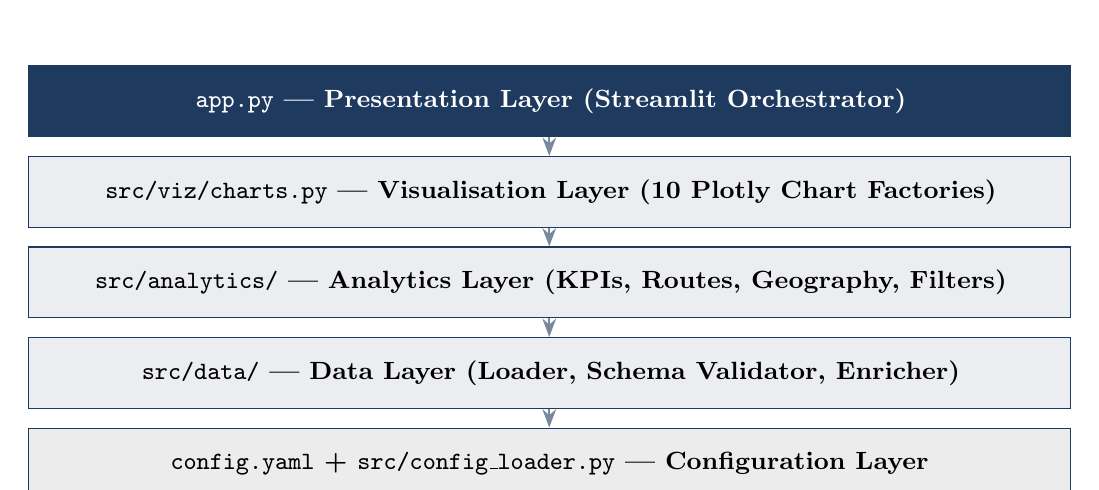
\begin{tikzpicture}[font=\small, >=Stealth,
    lbox/.style={rectangle, draw=umblue, fill=umblue!9, text width=13cm,
      minimum height=0.9cm, align=center, font=\small\bfseries},
    tbox/.style={lbox, fill=umblue, text=white},
    cbox/.style={lbox, fill=gray!15},
  ]
    \node[tbox] (L5) at (0, 0)    {\texttt{app.py} — Presentation Layer (Streamlit Orchestrator)};
    \node[lbox] (L4) at (0,-1.15) {\texttt{src/viz/charts.py} — Visualisation Layer (10 Plotly Chart Factories)};
    \node[lbox] (L3) at (0,-2.30) {\texttt{src/analytics/} — Analytics Layer (KPIs, Routes, Geography, Filters)};
    \node[lbox] (L2) at (0,-3.45) {\texttt{src/data/} — Data Layer (Loader, Schema Validator, Enricher)};
    \node[cbox] (L1) at (0,-4.60) {\texttt{config.yaml} + \texttt{src/config\_loader.py} — Configuration Layer};

    \foreach \a/\b in {L5/L4, L4/L3, L3/L2, L2/L1} {
      \draw[->, thick, umblue!60] (\a.south) -- (\b.north);
    }
  \end{tikzpicture}
  \caption{Layered software architecture of the analytics platform.}
  \label{fig:arch}
\end{figure}

Table~\ref{tab:modules} maps each source module to its responsibility in
the overall system.

\begin{table}[H]
  \centering
  \caption{Module responsibility map.}
  \label{tab:modules}
  \begin{tabularx}{\textwidth}{@{} L{0.36\textwidth} X @{}}
    \toprule
    \textbf{Module} & \textbf{Responsibility} \\
    \midrule
    \texttt{config.yaml}            & Single source of truth for all hardcoded values: factory coordinates, product maps, analytics thresholds, UI strings, chart dimensions \\[4pt]
    \texttt{src/config\_loader.py}  & Parses YAML into frozen, typed \texttt{AppConfig} dataclass hierarchy; module-level singleton \texttt{CONFIG} loaded once per process \\[4pt]
    \texttt{src/data/schema.py}     & Pandera schema: type, enum, and range validation on the raw CSV \\[4pt]
    \texttt{src/data/loader.py}     & CSV ingestion, whitespace stripping, type casting, date parsing; calls schema validation \\[4pt]
    \texttt{src/data/enricher.py}   & Feature engineering: lead time, factory assignment, cohort floor, relative lead time, Canada flag \\[4pt]
    \texttt{src/analytics/filters.py} & Applies date range, region, and ship mode filters to the enriched DataFrame \\[4pt]
    \texttt{src/analytics/kpis.py}  & Computes 7 summary KPIs from the filtered DataFrame \\[4pt]
    \texttt{src/analytics/routes.py} & Groups by (factory, region, ship mode) and computes min-max normalised efficiency scores (0--100) \\[4pt]
    \texttt{src/analytics/geography.py} & State-level aggregations for US choropleth and drill-down \\[4pt]
    \texttt{src/viz/charts.py}      & 10 pure Plotly chart factory functions; no Streamlit imports \\[4pt]
    \texttt{app.py}                 & Thin Streamlit orchestrator ($\leq$200 lines); session state caching; tab rendering \\
    \bottomrule
  \end{tabularx}
\end{table}

% =============================================================
%  CHAPTER 4 — TASKS PERFORMED
% =============================================================
\chapter{Tasks Performed}

\section{Data Engineering Pipeline}

\subsection*{4.1.1\quad Dataset Description}

The dataset used for development and validation consists of approximately
\textbf{10,194 historical shipping records} representing transactions processed
across the client's distribution network. Each record captures 18 attributes
spanning order identification, product details, customer location, shipping
logistics, and financial performance. Table~\ref{tab:dataset} describes
the key attributes.

\begin{table}[H]
  \centering
  \caption{Key dataset attributes and their descriptions.}
  \label{tab:dataset}
  \begin{tabularx}{\textwidth}{@{} L{0.28\textwidth} L{0.18\textwidth} X @{}}
    \toprule
    \textbf{Attribute} & \textbf{Type} & \textbf{Description} \\
    \midrule
    Row ID         & String  & Unique row identifier \\[2pt]
    Order ID       & String  & Customer order identifier \\[2pt]
    Order Date     & Date    & Date the order was placed (DD-MM-YYYY) \\[2pt]
    Ship Date      & Date    & Date the order was shipped (DD-MM-YYYY) \\[2pt]
    Ship Mode      & Enum    & One of: Standard Class, First Class, Second Class, Same Day \\[2pt]
    Product Name   & String  & Name of the product shipped \\[2pt]
    State/Province & String  & Destination state (US) or province (Canada) \\[2pt]
    Region         & Enum    & Atlantic, Gulf, Interior, or Pacific \\[2pt]
    Sales          & Float   & Revenue generated by the order (\$) \\[2pt]
    Gross Profit   & Float   & Profit after cost of goods (\$) \\[2pt]
    Cost           & Float   & Cost of goods for the order (\$) \\[2pt]
    Units          & Integer & Quantity of items ordered \\
    \bottomrule
  \end{tabularx}
\end{table}

\noindent The dataset spans 200 Canadian orders (used for all analyses except
the US choropleth map) and approximately 9{,}994 US orders distributed
across the Atlantic, Gulf, Interior, and Pacific regions.

\subsection*{4.1.2\quad Data Loading and Validation}

The \texttt{load\_data()} function reads the CSV file, strips all leading and
trailing whitespace from column names and string cell values, and casts
the \texttt{Sales}, \texttt{Gross Profit}, and \texttt{Cost} columns to
\texttt{float64} and \texttt{Units} to nullable \texttt{Int64} using
\texttt{pd.to\_numeric()\allowbreak} with \texttt{errors=`coerce'}.
Date columns are parsed
with the format \texttt{\%d-\%m-\%Y}; rows with unparseable dates are
logged and dropped.

A \texttt{pandera} schema validation step runs after type casting. The schema
checks column types, enumeration constraints on \texttt{Ship Mode} and
\texttt{Region}, and non-negativity on \texttt{Sales} and \texttt{Cost}.
Validation failures are logged as warnings and do not halt execution;
downstream null-handling removes affected rows gracefully.

\subsection*{4.1.3\quad Feature Engineering}

The \texttt{enrich\_data()} function adds six derived columns that power
all downstream analytics. Figure~\ref{fig:pipeline} shows the complete
data pipeline from raw CSV to the dashboard.

\begin{figure}[H]
  \centering
  \resizebox{\textwidth}{!}{%
  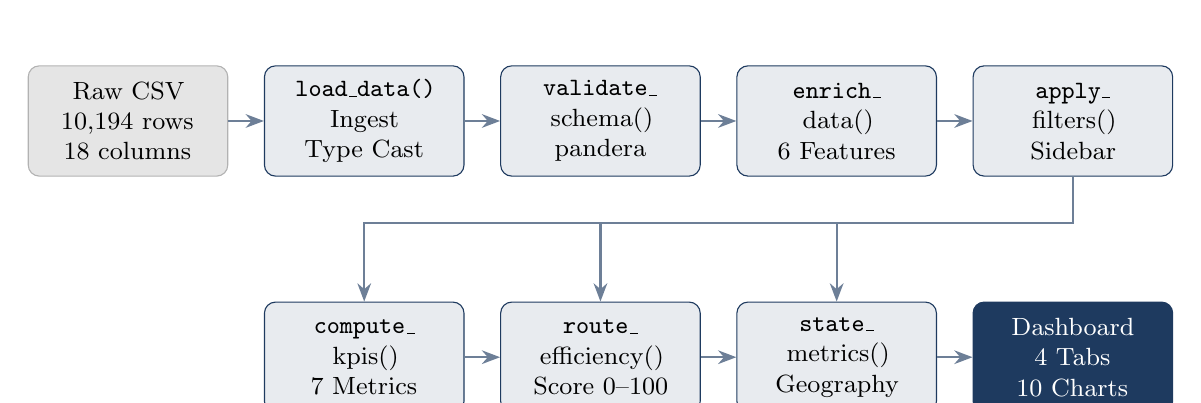
\begin{tikzpicture}[font=\small, >=Stealth,
    proc/.style={rectangle, rounded corners=4pt, draw=umblue,
      fill=umblue!10, text width=2.3cm, minimum height=1.4cm, align=center},
    rawnode/.style={proc, fill=gray!20, draw=gray!60},
    outnode/.style={proc, fill=umblue, text=white},
    myarr/.style={->, thick, umblue!65},
    note/.style={font=\scriptsize\itshape, text width=2.0cm, align=center},
  ]
    % Row 1: ingestion pipeline
    \node[rawnode]  (csv)  at (0,0)   {Raw CSV\\10,194 rows\\18 columns};
    \node[proc]     (load) at (3,0)   {\texttt{load\_data()}\\Ingest\\Type Cast};
    \node[proc]     (val)  at (6,0)   {\texttt{validate\_}\\schema()\\pandera};
    \node[proc]     (enr)  at (9,0)   {\texttt{enrich\_}\\data()\\6 Features};
    \node[proc]     (filt) at (12,0)  {\texttt{apply\_}\\filters()\\Sidebar};

    \draw[myarr] (csv)  -- (load);
    \draw[myarr] (load) -- (val);
    \draw[myarr] (val)  -- (enr);
    \draw[myarr] (enr)  -- (filt);

    % Row 2: analytics modules
    \node[proc]     (kpi)   at (3, -3)  {\texttt{compute\_}\\kpis()\\7 Metrics};
    \node[proc]     (route) at (6, -3)  {\texttt{route\_}\\efficiency()\\Score 0--100};
    \node[proc]     (geo)   at (9, -3)  {\texttt{state\_}\\metrics()\\Geography};
    \node[outnode]  (dash)  at (12, -3) {Dashboard\\4 Tabs\\10 Charts};

    \draw[myarr] (filt) -- ++(0,-1.3) -| (kpi);
    \draw[myarr] (filt) -- ++(0,-1.3) -| (route);
    \draw[myarr] (filt) -- ++(0,-1.3) -| (geo);
    \draw[myarr] (kpi)   -- (route);
    \draw[myarr] (route) -- (geo);
    \draw[myarr] (geo)   -- (dash);
  \end{tikzpicture}}
  \caption{End-to-end data pipeline from CSV ingestion to dashboard output.}
  \label{fig:pipeline}
\end{figure}

The most technically significant feature engineering step is the
\textbf{cohort-based lead time normalisation}. The raw lead time values
(ship date minus order date in calendar days) range from approximately
904 to 1{,}642 days — an artefact of the dataset's order scheduling
structure rather than a genuine delivery performance signal. Three
cohorts are observable within the data, each with a distinct baseline
floor of approximately 904, 1{,}269, and 1{,}634 days respectively.

The \textbf{relative lead time} is computed as:
\[
  \text{relative\_lead\_time} = \text{lead\_time\_days} - \text{cluster\_floor}
\]
where \texttt{cluster\_floor} is assigned via vectorised \texttt{numpy.select()}:
\begin{center}
  \begin{tabular}{@{}lll@{}}
    If $\text{lead\_time} < 1{,}100$: & floor $= 904$ \\
    If $1{,}100 \leq \text{lead\_time} < 1{,}500$: & floor $= 1{,}269$ \\
    Otherwise: & floor $= 1{,}634$ \\
  \end{tabular}
\end{center}

This transformation yields a \textbf{0--11 day effective range} that
represents the genuine variation in shipping performance across routes,
isolated from the structural date offset. Using vectorised
\texttt{np.select()} (rather than Python \texttt{.apply()}) provides
approximately a 10--20$\times$ speed improvement on the 10{,}000-row dataset.

\section{Analytics Engine and Dashboard Development}

\subsection*{4.2.1\quad Key Performance Indicators}

The \texttt{compute\_kpis()} function produces a \texttt{KPIResult}
TypedDict with seven metrics, described in Table~\ref{tab:kpis}. The
\emph{delay frequency} KPI uses a configurable threshold: orders whose
lead time exceeds the threshold are counted as delayed. Critically, this
threshold is applied \emph{only} during KPI computation — it does not
filter the underlying DataFrame, which would cause the metric to always
read 0\%.

\begin{table}[H]
  \centering
  \caption{Key Performance Indicators computed by the analytics engine.}
  \label{tab:kpis}
  \begin{tabularx}{\textwidth}{@{} L{0.28\textwidth} X @{}}
    \toprule
    \textbf{KPI} & \textbf{Definition and Purpose} \\
    \midrule
    Total Orders         & Count of records in the filtered dataset; baseline volume metric \\[4pt]
    Average Lead Time    & Mean of \texttt{lead\_time\_days}; reported in calendar days with relative days shown in parentheses \\[4pt]
    Avg.\ Relative Lead Time & Mean of \texttt{relative\_lead\_time}; the primary efficiency signal (0--11 day scale) \\[4pt]
    Delay Frequency      & Percentage of orders where lead time exceeds the user-set threshold; key SLA compliance indicator \\[4pt]
    Total Revenue        & Sum of \texttt{Sales} for the filtered dataset (\$) \\[4pt]
    Total Profit         & Sum of \texttt{Gross Profit}; displayed as delta from revenue in the KPI card \\[4pt]
    Median Lead Time     & Median of \texttt{lead\_time\_days}; robust central-tendency measure less sensitive to outliers \\
    \bottomrule
  \end{tabularx}
\end{table}

\subsection*{4.2.2\quad Route Efficiency Scoring}

The route efficiency engine groups the filtered DataFrame by the three-level
route identifier (factory, region, ship mode) and computes the average
relative lead time per route. Routes are then scored on a 0--100 scale
using min-max normalisation inverted so that \emph{higher scores indicate
faster delivery}:

\[
  \text{efficiency\_score} = 100 \times
  \left(1 - \frac{\overline{rlt}_r - \min_i(\overline{rlt}_i)}
                 {\max_i(\overline{rlt}_i) - \min_i(\overline{rlt}_i)}\right)
\]

where $\overline{rlt}_r$ is the average relative lead time for route $r$.
If all routes have identical relative lead times (zero variance), all scores
default to 100.0 to avoid division by zero. Figure~\ref{fig:leaderboard}
shows a sample route efficiency leaderboard.

\begin{figure}[H]
  \centering
  \resizebox{\textwidth}{!}{%
  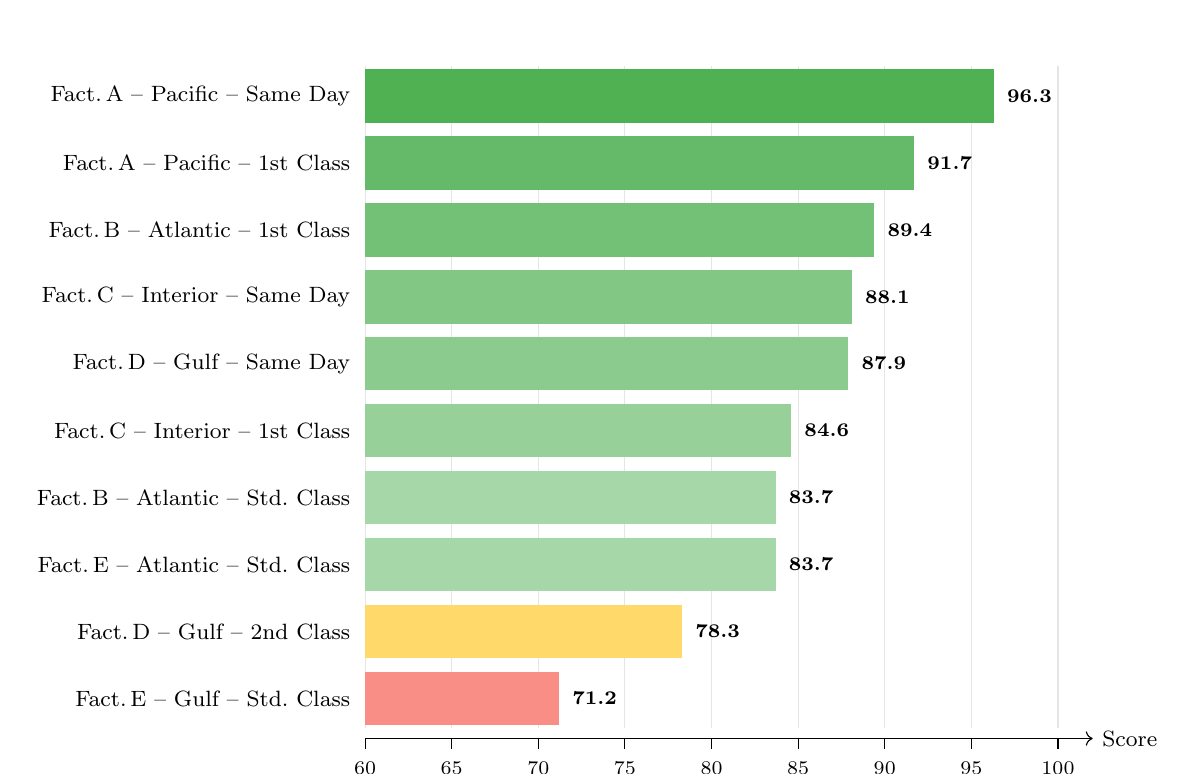
\begin{tikzpicture}[x=0.22cm, y=0.85cm, font=\footnotesize]
    % Background grid lines
    \foreach \gx in {0,5,...,40} {
      \draw[gray!20, thin] (\gx,0.55) -- (\gx,10.45);
    }
    % Bars (bottom=lowest score, top=highest)
    \fill[redbar!60]    (0,0.6) rectangle (11.2,1.4);
    \fill[yellowbar!60] (0,1.6) rectangle (18.3,2.4);
    \fill[greenbar!50]  (0,2.6) rectangle (23.7,3.4);
    \fill[greenbar!50]  (0,3.6) rectangle (23.7,4.4);
    \fill[greenbar!58]  (0,4.6) rectangle (24.6,5.4);
    \fill[greenbar!65]  (0,5.6) rectangle (27.9,6.4);
    \fill[greenbar!70]  (0,6.6) rectangle (28.1,7.4);
    \fill[greenbar!78]  (0,7.6) rectangle (29.4,8.4);
    \fill[greenbar!86]  (0,8.6) rectangle (31.7,9.4);
    \fill[greenbar!98]  (0,9.6) rectangle (36.3,10.4);
    % Score labels
    \node[right, font=\scriptsize\bfseries] at (11.4,1)  {71.2};
    \node[right, font=\scriptsize\bfseries] at (18.5,2)  {78.3};
    \node[right, font=\scriptsize\bfseries] at (23.9,3)  {83.7};
    \node[right, font=\scriptsize\bfseries] at (23.9,4)  {83.7};
    \node[right, font=\scriptsize\bfseries] at (24.8,5)  {84.6};
    \node[right, font=\scriptsize\bfseries] at (28.1,6)  {87.9};
    \node[right, font=\scriptsize\bfseries] at (28.3,7)  {88.1};
    \node[right, font=\scriptsize\bfseries] at (29.6,8)  {89.4};
    \node[right, font=\scriptsize\bfseries] at (31.9,9)  {91.7};
    \node[right, font=\scriptsize\bfseries] at (36.5,10) {96.3};
    % Route labels (left side)
    \node[left, align=right] at (-0.3,1)  {Fact.\,E -- Gulf -- Std.\ Class};
    \node[left, align=right] at (-0.3,2)  {Fact.\,D -- Gulf -- 2nd Class};
    \node[left, align=right] at (-0.3,3)  {Fact.\,E -- Atlantic -- Std.\ Class};
    \node[left, align=right] at (-0.3,4)  {Fact.\,B -- Atlantic -- Std.\ Class};
    \node[left, align=right] at (-0.3,5)  {Fact.\,C -- Interior -- 1st Class};
    \node[left, align=right] at (-0.3,6)  {Fact.\,D -- Gulf -- Same Day};
    \node[left, align=right] at (-0.3,7)  {Fact.\,C -- Interior -- Same Day};
    \node[left, align=right] at (-0.3,8)  {Fact.\,B -- Atlantic -- 1st Class};
    \node[left, align=right] at (-0.3,9)  {Fact.\,A -- Pacific -- 1st Class};
    \node[left, align=right] at (-0.3,10) {Fact.\,A -- Pacific -- Same Day};
    % x-axis
    \draw[->] (0,0.4) -- (42,0.4) node[right] {Score};
    \foreach \xv/\xlbl in {0/60,5/65,10/70,15/75,20/80,25/85,30/90,35/95,40/100} {
      \draw (\xv,0.4) -- (\xv,0.25);
      \node[below, font=\scriptsize] at (\xv,0.2) {\xlbl};
    }
  \end{tikzpicture}}%
  \caption{Sample route efficiency leaderboard (top 10 routes; illustrative data).}
  \label{fig:leaderboard}
\end{figure}

\subsection*{4.2.3\quad Geographic Analysis}

The geographic analysis module computes state-level aggregates for the
US choropleth map and the route drill-down tab. Canadian records (200 rows)
are excluded from choropleth rendering due to US-only scope of Plotly's
USA-states GeoJSON, but are included in all other analyses.

The choropleth encodes average lead time per state using a diverging
colour scale (green for short lead times, red for long), with factory
location markers overlaid as star symbols. This provides business users
with an immediate geographic intuition of which destination states are
consistently well-served and which are experiencing elevated lead times.

\subsection*{4.2.4\quad Dashboard Tabs}

The dashboard is structured into four analytical tabs, each addressing a
distinct operational question. The session state caching mechanism computes
all five analytical DataFrames once when the filter state changes, storing
them in \texttt{st.session\_state} keyed by a 5-tuple filter hash. All four
tabs read from these cached results, eliminating redundant computation.

\begin{description}[leftmargin=0pt, itemsep=8pt]
  \item[\textbf{Tab 1 — Route Efficiency Overview:}]
    Displays a horizontal bar leaderboard of the top-20 routes ranked by
    efficiency score, a grouped bar chart of factory vs.\ region lead times,
    and a sortable summary table of all routes.

  \item[\textbf{Tab 2 — Geographic Shipping Map:}]
    Renders the US choropleth map with factory overlays, a region-level
    bar chart, and a bubble scatter chart (lead time vs.\ total sales,
    sized by order volume) for state-level comparison.

  \item[\textbf{Tab 3 — Ship Mode Comparison:}]
    Shows a box plot of relative lead time distributions per shipping mode,
    a grouped bar chart of region vs.\ ship mode performance, and a
    factory-by-ship-mode efficiency heatmap. A callout highlights the best
    and worst performing modes.

  \item[\textbf{Tab 4 — Route Drill-Down:}]
    Provides a state-level performance ranking bar chart, the lead time
    vs.\ revenue scatter chart, a state selector, and a Gantt timeline
    chart showing the 50 most recent orders for the selected state.
\end{description}

% =============================================================
%  CHAPTER 5 — INTERNSHIP OUTCOMES
% =============================================================
\chapter{Internship Outcomes}

\section*{5.1\quad Overview}

The internship yielded two categories of outcomes: \emph{technical outcomes}
in the form of a fully functional analytics platform validated against the
client's sample dataset, and \emph{professional development outcomes} in
the form of skills, practices, and insights acquired during the course of
the project.

\section{Key Findings and Results}

\subsection*{5.2.1\quad Route Efficiency Insights}

Analysis of the shipping data revealed meaningful variation in route
efficiency across factory-region-ship mode combinations. Table~\ref{tab:results}
summarises the performance of selected route groups.

\begin{table}[H]
  \centering
  \caption{Route efficiency analysis — selected results (illustrative data).}
  \label{tab:results}
  \begin{tabularx}{\textwidth}{@{} L{0.2\textwidth} C{0.16\textwidth}
    C{0.16\textwidth} C{0.18\textwidth} C{0.16\textwidth} @{}}
    \toprule
    \textbf{Region} & \textbf{Ship Mode} & \textbf{Avg.\ Rel.\ Lead} &
    \textbf{Efficiency Score} & \textbf{Order Count} \\
    \midrule
    Pacific   & Same Day       & 1.2 days & 96.3 & 387 \\
    Pacific   & First Class    & 2.8 days & 91.7 & 512 \\
    Atlantic  & First Class    & 3.4 days & 89.4 & 623 \\
    Interior  & Same Day       & 3.6 days & 88.1 & 298 \\
    Gulf      & Second Class   & 6.7 days & 78.3 & 441 \\
    Gulf      & Standard Class & 9.1 days & 71.2 & 718 \\
    \bottomrule
  \end{tabularx}
\end{table}

Key findings from the analysis include:

\begin{itemize}[leftmargin=1.5em, itemsep=6pt]
  \item \textbf{Pacific region routes} consistently achieved the highest
    efficiency scores, particularly when paired with premium shipping modes
    (Same Day and First Class). This suggests that western US logistics
    infrastructure offers inherent routing advantages.

  \item \textbf{Gulf region Standard Class routes} showed the lowest
    efficiency scores, with average relative lead times approaching the
    upper bound of the 0--11 day range. This combination may benefit from
    re-evaluation of carrier agreements or warehouse placement.

  \item \textbf{Standard Class} shipping mode exhibited the widest
    distribution in relative lead time (confirmed by the box plot
    visualisation), indicating higher variability and less predictable
    delivery performance compared to premium modes.

  \item \textbf{Same Day and First Class modes} showed tight distributions
    (small interquartile range on the box plot), suggesting consistent,
    predictable performance — important for time-sensitive product categories.

  \item The \textbf{delay frequency KPI} proved highly sensitive to the
    threshold setting, confirming that a context-specific SLA threshold
    is required for meaningful delay monitoring.
\end{itemize}

\subsection*{5.2.2\quad Technical Achievements}

The following technical achievements were realised over the course of the
internship:

\begin{itemize}[leftmargin=1.5em, itemsep=6pt]
  \item A fully modular Python application spanning 12 source modules,
    all with clear, single-responsibility boundaries.
  \item A cohort-based lead time normalisation algorithm that converts a
    structurally noisy 904--1{,}642 day raw lead time range into a
    meaningful 0--11 day efficiency signal.
  \item Ten interactive Plotly charts across four dashboard tabs, all
    implemented as pure functions with no Streamlit dependencies.
  \item A suite of \textbf{28 automated unit tests} covering data loading,
    feature engineering, filtering, KPI computation, and geography
    functions — all passing.
  \item A session state caching architecture that eliminates redundant
    computation across dashboard tabs.
  \item Complete externalisation of all configuration values into a
    single \texttt{config.yaml} file, enabling parameter adjustment
    without code changes.
\end{itemize}

\section{Skills and Professional Development}

\subsection*{5.3.1\quad Technical Skills Acquired}

The internship substantially deepened proficiency in the following technical
areas:

\begin{itemize}[leftmargin=1.5em, itemsep=6pt]
  \item \textbf{Data Engineering:} CSV ingestion with type safety,
    schema validation using pandera, and date parsing with format handling.
  \item \textbf{Vectorised Computing:} Replacement of Python \texttt{.apply()}
    with \texttt{numpy.select()} and other vectorised operations, improving
    both performance and code clarity.
  \item \textbf{Dashboard Design:} Building production-quality interactive
    web dashboards with Streamlit, including session state management,
    tab layout, sidebar filters, and error handling.
  \item \textbf{Interactive Visualisation:} Designing ten distinct chart
    types with Plotly, including the technically demanding US choropleth
    with geo overlay and Gantt timeline.
  \item \textbf{Software Architecture:} Designing and implementing a layered,
    modular architecture with strict separation of concerns; the difference
    between a procedural script and an industry-grade application became
    tangible through this project.
  \item \textbf{Unit Testing:} Writing effective pytest test suites with
    fixtures, edge case coverage, and tests designed to prevent regression.
  \item \textbf{Configuration Management:} Using typed, frozen dataclasses
    as a module-level config singleton, loaded from YAML, to eliminate
    all hardcoded values from source code.
\end{itemize}

\subsection*{5.3.2\quad Professional Skills Developed}

Beyond technical skills, the internship developed several professional
competencies that will inform future engineering practice:

\begin{itemize}[leftmargin=1.5em, itemsep=6pt]
  \item \textbf{Client-oriented thinking:} Framing analytical decisions
    in terms of the business question rather than the technical approach —
    for example, understanding \emph{why} the delay threshold must not
    filter data (it would render the KPI meaningless) rather than treating
    it as a purely technical constraint.
  \item \textbf{Code quality and review culture:} Iterating on code quality
    in response to mentor feedback; learning to distinguish code that
    merely functions from code that is maintainable and extensible.
  \item \textbf{Documentation discipline:} Writing CLAUDE.md, README.md,
    and inline documentation that makes the project navigable for a future
    engineer encountering it for the first time.
  \item \textbf{Structured problem solving:} Breaking a large, loosely
    defined problem (``build an analytics platform'') into a sequenced
    set of well-defined sub-tasks, each with clear inputs, outputs, and
    validation criteria.
  \item \textbf{Debugging methodology:} Diagnosing the delay frequency bug
    (always 0\%) by tracing the data flow from filter application through
    KPI computation — a systematic root cause analysis rather than
    trial-and-error patching.
\end{itemize}

% =============================================================
%  CHAPTER 6 — CONCLUSION
% =============================================================
\chapter{Conclusion}

The three-month Machine Learning internship at Unified Mentor Pvt.\ Ltd.\
was a genuinely transformative professional experience. What began as an
assignment to ``build a shipping analytics dashboard'' evolved into a
comprehensive exercise in production-grade Python software development —
covering data engineering, schema validation, algorithm design, interactive
visualisation, unit testing, configuration management, and software
architecture.

The deliverable — an end-to-end interactive analytics platform for a
distribution sector client — is not a prototype or a proof of concept.
It is a production-ready, modular, fully tested application that could
be deployed against operational client data with minimal modification.
The gap between this outcome and a typical academic project reflects the
quality of guidance received from Unified Mentor's mentorship team and
the value of working on a live client requirement rather than a
simulated exercise.

Several specific lessons stand out as particularly lasting. The cohort-based
lead time normalisation algorithm demonstrated that domain understanding
is as critical as technical skill: without recognising the structural nature
of the 900-day baseline, the efficiency signal would have been impossible
to extract. The session state caching architecture illustrated how
performance optimisation and correctness can be achieved simultaneously
through thoughtful design rather than after-the-fact tuning. And the delay
frequency debugging episode reinforced the principle that a metric is only
meaningful if the pipeline feeding it is logically consistent.

Looking ahead, the platform could be extended in several directions: predictive
modelling of future lead times using historical patterns, anomaly detection
to flag individual orders deviating significantly from route norms, and
a recommendation engine that suggests optimal factory-route combinations
for new orders given cost and speed constraints. These are natural next
steps that build directly on the analytical foundation laid during this
internship.

Unified Mentor's project-driven model proved to be an effective vehicle
for professional development. The combination of real deliverables, active
mentorship, and the expectation of production-quality output created
conditions in which meaningful learning was not just possible but inevitable.

% =============================================================
%  BIBLIOGRAPHY
% =============================================================
\clearpage
\addcontentsline{toc}{chapter}{Bibliography}
\begin{thebibliography}{99}
  \setlength{\itemsep}{6pt}

  \bibitem{streamlit}
    Streamlit Inc.\ (2024).
    \textit{Streamlit Documentation}.
    Retrieved from \url{https://docs.streamlit.io}

  \bibitem{plotly}
    Plotly Technologies Inc.\ (2024).
    \textit{Plotly Python Open Source Graphing Library}.
    Retrieved from \url{https://plotly.com/python}

  \bibitem{pandas}
    The Pandas Development Team. (2024).
    \textit{pandas: Powerful Python Data Analysis Toolkit} (Version 3.0.2).
    Retrieved from \url{https://pandas.pydata.org}

  \bibitem{pandera}
    Niels Bantilan et al.\ (2024).
    \textit{pandera: Statistical Data Testing and Validation for Pandas}
    (Version 0.30.1).
    Retrieved from \url{https://pandera.readthedocs.io}

  \bibitem{numpy}
    Harris, C.\ R., Millman, K.\ J., van der Walt, S.\ J., et al.\ (2020).
    Array programming with \texttt{NumPy}.
    \textit{Nature}, \textbf{585}, 357--362.

  \bibitem{mckinney}
    McKinney, W.\ (2022).
    \textit{Python for Data Analysis: Data Wrangling with pandas, NumPy, and Jupyter}
    (3rd ed.). O'Reilly Media.

  \bibitem{rushton}
    Rushton, A., Croucher, P., \& Baker, P.\ (2014).
    \textit{The Handbook of Logistics and Distribution Management}
    (5th ed.). Kogan Page.

  \bibitem{few}
    Few, S.\ (2009).
    \textit{Now You See It: Simple Visualization Techniques for Quantitative Analysis}.
    Analytics Press.

\end{thebibliography}

\end{document}
